The thresholding bandit problem is a specific instance of the pure-exploration setup of \citet{chen2014combinatorial}. To put it in perspective, the considered TBP setup lies at the intersection of the larger pure exploration setting and the stochastic multi-armed bandit (SMAB) setting discussed in chapter \ref{chap:SMAB} and chapter \ref{chap:EUCBV}. This is shown in Figure \ref{fig:con}.

\begin{figure}[!th]
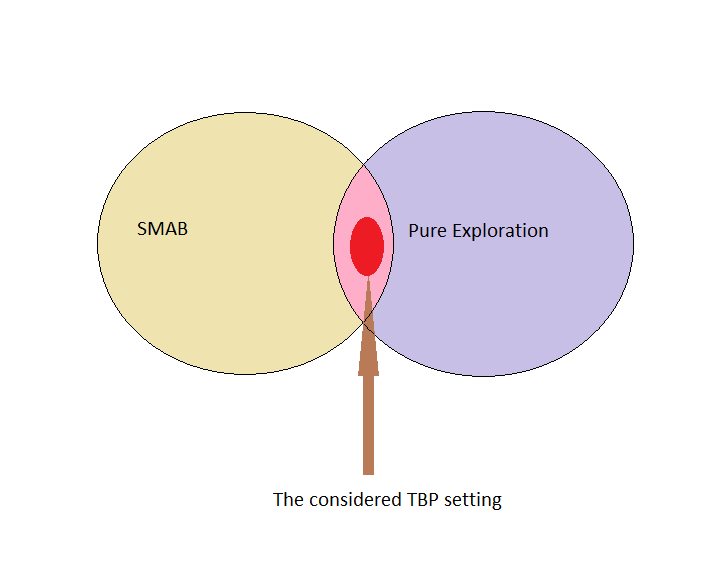
\includegraphics[scale=0.7]{Chapter4/img/connection_TBP.png}
\caption{Connection between TBP, Pure Exploration and SMAB}
\label{fig:con}
\end{figure}

\subsubsection{Challenges in the TBP seeting}

Further, if we look closely into the TBP setting we will see that there are several similarities between the challenges in SMAB setting and the TBP setting. These challenges are as follows:-

\begin{enumerate}
\item Closer an arm’s expected reward mean ($r_i$) to $\tau$ $\Rightarrow$ Harder is the problem. This stems from the fact that it becomes increasingly difficult to discriminate between the arms lying above and below $\tau$.
\item Lesser the budget $T$ $\Rightarrow$ Harder is the problem. This is because there are lesser number of pulls available and so the number of samples collected tends to be low.
\item Higher the variance of an arm’s reward distribution $D_i$ $\Rightarrow$ Harder is the problem. This is similar to the first case as it becomes harder to discriminate between the arms lying close to the threshold.
\end{enumerate}

In the theoretical section in chapter \ref{chap:tbandit2} we will try to characterize this hardness and give guarantees that are almost optimal.